% Template for white paper submissions for the 
% LSST Call for Observing Strategies for DeepDrilling and Minisurveys 
% 
% The call for white papers can be found at https://github.com/lsst-pst/survey_strategy/blob/master/latex/WPcall2018.pdf
% The deadline for submissions is November 29, 2018
%  To submit white papers, please email the compiled PDF to lsst-survey-strategy@lists.lsst.org   
%   subdirectory named LASTNAME_FIRSTNAME_NUMBER	%  OR submit a pull request to this github repository (github.com/lsst-pst/survey_strategy_wp) with your white paper in a clearly named subdirectory.
% For help with white papers or the submission process, please post at http://community.lsst.org/c/sci/survey-strategy



\documentclass[12pt, letterpaper]{article}
\usepackage[top=1in, bottom=1.5in, left=1in, right=1in]{geometry}
\usepackage[utf8]{inputenc}
\usepackage{aas_macros}
\usepackage{booktabs}
\usepackage{hyperref}
\usepackage{color}
\usepackage{graphicx}
\usepackage{caption}
\usepackage{lineno}
\linenumbers

\newcommand{\ml}[1]{{\textcolor{blue}{#1}}}
\newcommand{\review}[1]{{\textcolor{red}{#1}}}
\newcommand{\reviewnew}[1]{{\textcolor{magenta}{#1}}}
\def\subsectionautorefname{Sec}
\def\sectionautorefname{Sec}

\title{LSST DESC WFD Survey Optimization \\(White Paper)}
%EG added parentheses in title
\author{}
\date{November 2018}

\begin{document}


\maketitle

\begin{abstract}
Cosmology is one of the cornerstones of LSST, which promises to be transformative for our understanding of dark energy and dark matter. However, each of the cosmological probes for LSST is heavily impacted by the choice of observing strategy.
This white paper is the result of efforts by the LSST DESC Observing Strategy Task Force (OSTF), which represents the entire collaboration, and aims to make recommendations on observing strategy that will benefit all cosmological analyses with LSST. It should be accompanied by the DESC DDF white paper (Scolnic et al.). We use a variety of metrics to understand the effects of the observing strategy on measurements of weak lensing, large-scale structure, clusters, photometric redshifts, supernovae, strong lensing and kilonovae. \review{In order to reduce systematic effects,} we conclude that the baseline observing strategy needs to be significantly improved to result in \review{the best possible} cosmological constraints.  
Our key recommendations include: moving the WFD footprint to a lower extinction region, taking visit pairs in different filters, changing the 2$\times$15s snaps to single exposures to improve efficiency, focusing on strategies that reduce long gaps ($>$15 days) between observations, and prioritizing spatial uniformity at several intervals during the 10-year survey.
%EG added that last one
\end{abstract}

\newpage
\section{White Paper Information}
Michelle Lochner, \url{dr.michelle.lochner@gmail.com}\\
Dan Scolnic, \url{dscolnic@kicp.uchicago.edu}\\
On behalf of the LSST Dark Energy Science Collaboration (DESC) %EG Observing Strategy Task Force
\\

\begin{enumerate} 
\item {\bf Science Category:}\\
Constraining dark energy and dark matter.\\
Exploring the transient optical sky (especially supernovae and kilonovae).\\
\item {\bf Survey Type Category:}\\
    Wide-fast-deep
\item {\bf Observing Strategy Category:}\\ 
An integrated program with science that hinges on the combination of pointing and detailed 
	observing strategy - we propose a set of factors crucial for an observing strategy optimized for cosmology.
\end{enumerate}  


\clearpage

\section{Scientific Motivation}

% \begin{footnotesize}
% {\it Describe the scientific justification for this white paper in the context
% of your field, as well as the importance to the general program of astronomy, 
% including the relevance over the next decade. 
% Describe other relevant data, and justify why LSST is the best facility for these observations.
% (Limit: 2 pages + 1 page for figures.)}
% \end{footnotesize}

\subsection{Introduction}
Providing cutting-edge constraints on dark matter and dark energy models is one of the key science goals of LSST. The infographic in \autoref{fig:infographic} illustrates the wide array of cosmological probes that LSST will revolutionize. The ability to take almost all the observations required with the same instrument, as well as having a large enough dataset to subdivide repeatedly, will minimize the systematic effects that can dominate cosmological constraints. \autoref{fig:contours} shows the expected constraints from \emph{LSST data alone}. In addition to being world-leading in the cosmological probes \review{of weak lensing, large scale structure, clusters and supernovae}, LSST also will allow completely novel studies such as testing homogeneity and isotropy and the use of rare objects like kilonovae and strongly lensed supernovae for independent cosmological constraints. It will provide an enduring legacy dataset of galaxies and transient events that will be studied for decades. However, all this will only be possible if the observing strategy of LSST is carefully optimized. Here we briefly summarize the main cosmological probes of LSST, separated into ``static science'' and ``transient science'', as the probes within these two categories have broadly similar observing strategy requirements. Of special consideration are photometric redshifts, which are critical in enabling all other cosmological probes, since spectroscopic follow-up for all galaxies and transients will be impossible. Thus we consider in this paper the effect of observing strategy on photometric redshifts, which rely on obtaining sufficient depth in the $ugriz$ \review{filter set} across the footprint.

\subsection{Static Science}

\hspace{\parindent}{\bf Weak Lensing}\\
The sample of billions of galaxies produced by LSST will be by far the largest of its time \cite{lsst2009}. It will enable unprecedented constraints from weak lensing, one of the most powerful and direct probes of cosmology. Systematic effects rather than statistical noise will \review{be of critical importance} and with its high image quality and large data volumes, LSST is the best experiment for understanding and mitigating these effects. As well \review{having similar} depth and area requirements of large-scale structure measurements, weak lensing additionally requires a high number of visits for accurate PSF estimation and other systematic effects.\\

\hspace{\parindent}{\bf Large-Scale Structure and Galaxy Clusters}\\
%EG lacking a separate Clusters sub-section, this points people looking for that probe to here
 The same enormous dataset of galaxies will allow the use of cutting-edge analysis techniques, such as galaxy-galaxy correlations, \review{cross-correlation with weak lensing}, counts of galaxy clusters, and cross correlation with the CMB \cite{lsst2009}. Large-scale structure studies will place constraints on primordial fluctuations that are competitive with the CMB and will allow stringent tests of non-Gaussianity. Achieving these science goals will require surveying a large area with low extinction and uniform depth to mitigate systematics. \review{Cluster counts are a powerful probe of cosmology that are included in our analysis and have similar requirements to weak lensing and large scale structure.} \\



\subsection{Transient Science}
\hspace{\parindent}{\bf Supernovae}\\
LSST will deliver hundreds of thousands of \review{type Ia} supernovae, the exact number being highly dependent on observing strategy, allowing unprecedented tests of cosmology with supernovae alone \cite{lsst2009}.
%EG I left the following alone, but SN are not the only probe that lest us test homogeneity/isotropy, and that was already mentioned generically in the Introduction.  
The large sample will enable tests of homogeneity and isotropy, as well as the study of supernova evolution and systematics as a function of redshift, galaxy type, environment and supernova properties. However, \review{this requires well-measured light curves that are high enough cadence to classify them as type Ia and obtain distances from them. Thus,} supernova studies with WFD is one of the cosmological probes most sensitive to choice of observing strategy, requiring regular cadence, frequent filter changes (for instance ensuring visit pairs in a night are in different filters) and a season length of about 5 months.\\

{\bf Strong Lensing}\\
Strongly lensed \review{objects} are both faint and rare, making them difficult to detect in most surveys. The LSST WFD survey, however, will be able to detect a large number of strongly lensed quasars and supernovae, allowing not only independent tests of cosmology, but also novel extragalactic studies. Lensed quasars and supernovae allow a unique test of distance-duality, one of the fundamental relations in cosmology, as well as independent constraints on the much-contested value of $H_0$. Maximising the number of strongly lensed supernovae detected would require long cumulative season lengths and good cadence.\\

{\bf Gravitational Waves}\\
After the first detection of a binary neutron star merger in 2017, multi-messenger astronomy is quickly emerging as an exciting scientific discipline. LSST will detect more kilonovae than any other experiment of its time \cite{scolnic2017}, making it the best facility for serendipitous kilonova detections. Combined with observations from gravitational wave detectors, kilonovae \review{are a promising probe that could} constrain the expansion history of the universe in a way that is complementary to other probes. Similar to supernovae, detecting kilonovae will require regular cadence with frequent filter changes.

\newpage
\begin{center}
\begin{minipage}{0.99\columnwidth}
    \centering
    \includegraphics[width=0.8\columnwidth]{DESC_footprint2.pdf}
    \captionof{figure}{Infographic showing the impressive range of cosmological probes for which LSST will be transformative.}
    \label{fig:infographic}
\end{minipage}
\vspace{20pt}

\begin{minipage}{0.99\columnwidth}
    \centering
    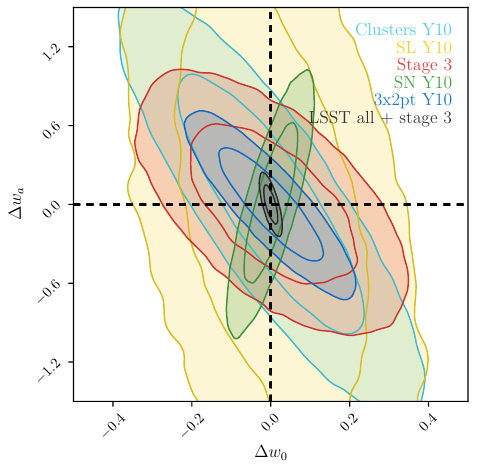
\includegraphics[width=0.6\columnwidth]{desc_srd_constraints.png}
    \captionof{figure}{Expected 10 year constraints on time-varying dark energy combining all LSST cosmological probes, from the DESC SRD \cite{descsrd}. The contours labeled Stage 3 represents combined current constraints from the CMB, baryon acoustic oscillations, and supernovae. LSST will clearly constitute a vast improvement over the current state of the art. \review{Especially note the complimentarity of the static science and transient science probes required to break degeneracies in cosmological constraints: if observing strategy is not optimized for both sets of probes, cosmology with LSST will be limited by these degeneracies.}}
    \label{fig:contours}
\end{minipage}
\end{center}

\vspace{.6in}

\section{Technical Description}
% \begin{footnotesize}
% {\it Describe your survey strategy modifications or proposed observations. Please comment on each observing constraint
% below, including the technical motivation behind any constraints. Where relevant, indicate
% if the constraint applies to all requested observations or a specific subset. Please note which 
% constraints are not relevant or important for your science goals.}
% \end{footnotesize}

\subsection{High-level description}
% \begin{footnotesize}
% {\it Describe or illustrate your ideal sequence of observations.}
% \end{footnotesize}
\review{In \autoref{tab:obs_constraints} we indicate the most important factors to ensure a successful cosmology program with LSST.} Here, we highlight several important changes to observing strategy that would enable the best possible cosmological constraints from LSST. 
\begin{itemize}
    \item To improve all extragalactic science, we propose to move the 18,000 square degree WFD footprint away from the galactic plane to avoid the zone of high extinction.  \review{Galactic science has different observing strategy needs to extragalactic science, so we propose to} expand the Galactic plane mini-survey and optimize its cadence and filter choices for Milky Way science, including a microlensing survey to probe dark matter properties.    
\item We stress that uniformity in co-added depth across the entire WFD footprint is critical for cosmology and must be achieved after Y1, Y10 and at 2-3 reasonable intervals in between for data releases (here we use Years 1,3,6,10). 
\item \review{To obtain high enough quality light curves for photometric classification of supernovae and for accurate distance measures,} we require a mean cadence of 10(g),5(r),6(i),6(z) days, with no long gaps ($>15$ days in any given filter) between observations.\review{A strategy that achieves this results in more than twice as many well-characterized supernovae over the baseline strategy (see \autoref{fig:transients}).} \review{In addition, we recommend a single exposure instead of the 2$\times$15s snaps. Although the optimal exposure time is yet to be determined, 30s will likely be near optimum}.
\item Nightly visit pairs should be in neighboring filters instead of the same filter. 
\item Longer season lengths\review{\footnote{A season length is how long a field is observable in a year. It is largely dictated by the field's declination but can be shortened in observing strategies where low airmass is prioritized}} are preferred, but not at the expense of the requested cadence. 
\item We \review{are interested in exploring the possibility of} redistributing roughly half of the $y$-band visits into $griz$. 
\item We note that rolling cadence may be required to achieve this cadence but more study is needed to determine this. 
\item Finally, we find that results from AltSched, an alternative scheduler to OpSim, show that it is a highly promising approach and recommend exploring its scheduling methods in OpSim and especially comparing it to the new feature-based scheduler\footnote{\review{The feature-based scheduler \cite{feature2018} uses a modified Markov decision process to choose observations on-demand, while the current OpSim proposal-based scheduler \cite{opsim2014} attempts to execute a predefined list of observations, similar to traditional manual telescope scheduling of proposals from various astronomers.}} (see \autoref{sec:requests}).
\end{itemize}

\vspace{.3in}

\subsection{Footprint -- pointings, regions and/or constraints}
\label{sec:footprint}
% \begin{footnotesize}{\it Describe the specific pointings or general region (RA/Dec, Galactic longitude/latitude or 
% Ecliptic longitude/latitude) for the observations. Please describe any additional requirements, especially if there
% are no specific constraints on the pointings (e.g. stellar density, galactic dust extinction).}\\
% \end{footnotesize}
All cosmological probes require observations at low \review{galactic} extinction. Therefore, we strongly recommend selecting an 18,000 deg$^2$  footprint based on a E(B-V)$<0.2$ cut \review{(in this analysis derived from SFD maps and converted to E(B-V) using MAF)}. \autoref{fig:footprint} shows our proposed footprint in a declination range of $-70<$dec$<12.5$, chosen based on the extinction cut and to improve overlap with 4MOST for spectroscopic follow-up. Our studies have shown that with the current WFD footprint, 25\% of the area is \review{unsuited for cosmology}. With our new proposed footprint, we will obtain considerable additional area \review{for extragalactic science} at no cost to depth. \review{It can be seen in \autoref{fig:static_fom} that the larger area simulations such as \texttt{pontus\_2002} result in $\sim30\%$ more area which corresponds to a $\sim20\%$ improvement in dark energy constraints. However, the larger area surveys have worse constraints on systematics so we recommend to rather optimize the existing footprint than increase the survey area. Determining the precise area that optimizes the trade-off between statistical and systematic errors is ongoing work.} It is also important to ensure that the WFD has good spatial and temporal 
overlap with spectroscopic survey instruments, especially 4MOST and DESI, to obtain spectroscopic redshifts and classifications of a sufficient training set of objects.\\ 

\begin{minipage}{\columnwidth}
\centering
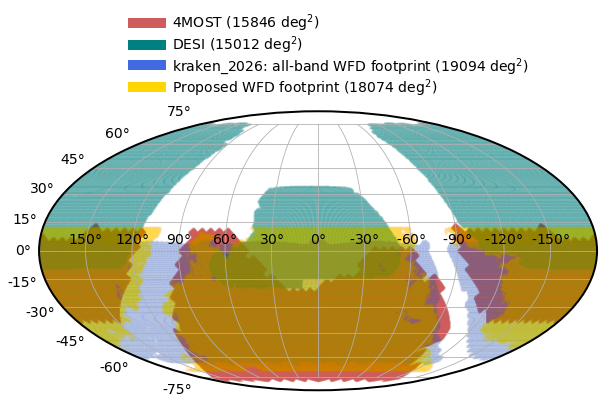
\includegraphics[width=0.8\columnwidth]{wfdfootprint_proposed_vs_kraken_2026_vs_4most_desi_nside256_matplotlib.png}
 \captionof{figure}{Proposed WFD footprint based on an E(B-V)$<0.2$ cut (yellow), the baseline footprint (blue) and the DESI (green) and 4MOST (red) footprints.}  \label{fig:footprint}
\end{minipage}
%EG mentioned this above so commented out here
%We note that microlensing for dark matter studies is an interesting probe that will benefit from a well-designed galactic plane mini survey rather than galactic observations in WFD, thus we do not consider it here.\\

\subsection{Image quality}
\label{sec:image_quality}
% \begin{footnotesize}
% {\it Constraints on the image quality (seeing).}\\
% \end{footnotesize}
Weak lensing and other science probes have stringent requirements on image quality, \review{especially in $r$ and $i$}. To produce the highest quality images, we recommend scanning along the meridian as 
much 
as possible. However, this should generally not come at the cost of season length, which impacts transient science. Further potential optimizations to image quality include prioritizing certain filters in the best seeing conditions and varying exposure time based on observing conditions. These are described in \autoref{sec:requests}.

\subsection{Individual image depth and/or sky brightness}
% \begin{footnotesize}{\it Constraints on the sky brightness in each image and/or individual image depth for point sources.
% Please differentiate between motivation for a desired sky brightness or individual image depth (as 
% calculated for point sources). Please provide sky brightness or image depth constraints per filter.}\\
% \end{footnotesize}
A positive detection of supernovae requires a reasonably good single visit depth and the $5\sigma$ \review{point source detection} canonical baseline numbers \review{from the LSST SRD \cite{lsstSRD}} should be used as guidelines (g:24.6, r:24.3, i:23.6, z:22.9). %Single visit depth is less important for static science, as long as the images are not readnoise limited. 
%EG***  Can this be motivated based on the desired median redshift for SN, which trades off against the number of SN?    

\subsection{Co-added image depth and/or total number of visits}
% \begin{footnotesize}{\it  Constraints on the total co-added depth and/or total number of visits.
% Please differentiate between motivations for a given co-added depth and total number of visits. 
% Please provide desired co-added depth and/or total number of visits per filter, if relevant.}\\
% \end{footnotesize}
To achieve our goals with weak lensing, large-scale structure and clusters, we require a co-added depth of $i>24.5$ for Y1 and $i>26.0$ for Y10. 
%EG Achieving 
Approaching 
sufficient co-added depth for $ugriz$ across the entire footprint is critical for photometric redshifts, whilst  $y$  is somewhat less important (see \autoref{sec:filters}). The total number of visits is important to reduce weak lensing systematics (such as PSF modeling), that
average down as a function of the number of visits. For transient-based cosmology, the cadence of visits across $griz$ is much more important than the total number. Thus we recommend as large a number of visits as possible, \emph{only after all other requirements on co-added depth and cadence are met.}

\subsection{Number of visits within a night}
% \begin{footnotesize}{\it Constraints on the number of exposures (or visits) in a night, especially if considering sequences of visits.  }\\
% \end{footnotesize}
\review{We strongly recommend visit pairs be in different, neighboring filters as this} improves cadence and thus supernova cosmology. The effect of removing the visit pairs can be seen by comparing \texttt{colossus\_2667} with the baseline \texttt{kraken\_2026} in \autoref{fig:transients}, where all metrics are improved. However, because the study of asteroids is both an important LSST science case and is critical for removing false positives in extragalactic transient classification, we propose maintaining the visit pairs requirement but we strongly recommend performing the visits in different (neighboring) filters. This would also dramatically improve early transient classification. \emph{The loss of regular cadence due to multiple visits to the same field in a single night in the same filter would be highly damaging for cosmology.} 
%EG added emphasis above

\subsection{Distribution of visits over time}
\label{sec:cadence}
% \begin{footnotesize}{\it Constraints on the timing of visits --- within a night, between nights, between seasons or
% between years (which could be relevant for rolling cadence choices in the WideFastDeep. 
% Please describe optimum visit timing as well as acceptable limits on visit timing, and options in
% case of missed visits (due to weather, etc.). If this timing should include particular sequences
% of filters, please describe.}\\
% \end{footnotesize}
\review{To make optimal use of LSST for supernova cosmology, we recommend a minimum mean cadence of 10($g$), 5($r$), 6($i$), 6($z$) days. This recommendation is significantly higher cadence than \texttt{kraken\_2026} (22($g$), 12($r$), 12($i$), 14($z$)) but still less than the highest performing strategy, \texttt{alt\_sched\_rolling} (8($g$), 3($r$), 4($i$), 3($z$)). Early classification of supernovae requires at least two points in different colors in the rise of the light curve. We find that this is achievable with our recommended cadence for all observable SNe below $z=0.25$ (dropping off at around $z=0.4$ whereas \texttt{kraken\_2026} detects less than two points on the rise for more than 50\% of SNe making, early classification impossible.} \\

\noindent
However, average cadence is not the only consideration. Long gaps ($>$15 days) between observations in a season critically need to be avoided (see \autoref{fig:transients}). The distribution of inter-night gaps needs to be narrow, as well as have a low average, to achieve excellent transient science results. Thus the filters should be cycled through as much as possible to create an even cadence. To accommodate rare, slowly varying transients such as strongly lensed supernovae, longer season lengths (at least 5 months) are preferred as long as this cadence is achieved.\\ 

\noindent
\review{To avoid negatively impacting static science, any rolling cadence must provide uniformity at the selected intervals (for example, Y1, Y3, Y6, Y10). \emph{Rolling cadence is thus only preferred if it is necessary to achieve the above cadence requirements.} While we do not currently have access to enough accurate rolling cadence simulations to draw definitive conclusions, we remain very interested in continuing to investigate it as a potential strategy.}

\subsection{Filter choice}
\label{sec:filters}
% \begin{footnotesize}
% {\it Please describe any filter constraints not included above.}\\
% \end{footnotesize}
We are interested in investigating a change in the distribution of visits per filter. It is expected that a bluer distribution of filters would improve the number of high quality supernovae detected, without impacting static science. See \autoref{sec:requests} for a description of our proposed strategy. \review{The filters $griz$ are all critically important for supernovae so should be regularly cycled through. $u$-band is very important for photometric redshifts, while it may be less important to obtain the same depth in $y$ \cite{graham2017}}.

\subsection{Exposure constraints}
% \begin{footnotesize}
% {\it Describe any constraints on the minimum or maximum exposure time per visit required (or alternatively, saturation limits).
% Please comment on any constraints on the number of exposures in a visit.}\\
% \end{footnotesize}
We strongly support dropping the 2$\times$15s snaps in favor of a single exposure as this increases observing efficiency while allowing a slower readout during slew, which will improve camera performance.  \review{Rough calculations indicate the efficiency increases by about 7\%, which is significant given that (for example) the entire DDF programme is only 5\% of the observing time. This extra efficiency could be used to improve the cadence by increasing the number of inter-night visits. \review{Our analysis also indicates that it is unlikely that single 30s exposures will cause saturation for more than a small number of very nearby supernovae and so is still worth the efficiency gain.} While cosmic rays have been successfully removed in single exposures without snaps (e.g. with Hyper Suprime-Cam \cite{aihara2017}), we acknowledge that image simulations would be important to ensure this can effectively be done with LSST}.\\ 
In our study, we found that \texttt{pontus\_2489} (an OpSim run with 20s exposures in $grizy$ and 40s in $u$) performed well for weak lensing systematics and did not decrease the depth and area. The sample of transients is larger but at a lower redshift on average. We thus need further investigation to determine the optimal exposure time. 
We would also be interested in exploring variable exposures as described in \autoref{sec:requests}. 

\subsection{Other constraints}
% \begin{footnotesize}
% {\it Any other constraints.}\\
% \end{footnotesize}
\begin{itemize}
\item {\bfseries Dithering: }Dithering is critical to delivering excellent 
%EG added 
calibration and 
cosmological constraints with LSST. We recommend random translational dithers of amplitude 0.5*FOV for WFD with a single dither vector used on each night \cite{awan2016, carroll2014}.  We note that translational dithering can also be achieved with a no-fixed field strategy that re-tesselates the sky each night (such as the feature-based scheduler or AltSched). \review{We also recommend that nightly rotational dithers be performed by choosing a single RotTelPos value randomly, returning to this value after each filter change and then controlling instrument rotation such that all re-visits to individual fields are performed at the same value of RotSkyPos.} 
\item {\bfseries Uniformity: }\review{We measure uniformity as the standard deviation of the $5\sigma$ $i$-band depth across the sky (after a depth cut). The Y10 uniformity of the baseline strategy \texttt{kraken\_2026} ($0.13$ mag) is sufficient, but we note that several strategies such as \texttt{mothra\_2045} are a factor of 2 less uniform, while AltSched results in a roughly 20\% improvement. Uniformity should be checked using this metric for key release years.}

\end{itemize}
\subsection{Estimated time requirement}
% \begin{footnotesize}
% {\it Approximate total time requested for these observations, using the guidelines available at \url{https://github.com/lsst-pst/survey_strategy_wp}.}\\
% \end{footnotesize}
We request that WFD utilize at least 80\% of total observing time
in order to achieve the LSST SRD requirement of a median of 825 visits over at least 18,000 deg$^2$ along with our science goals.  
%EG added previous phrase and edited the following sentence
As our new proposed WFD footprint would exclude the galactic plane, we expect that the Galactic Plane mini-survey will require increased time to achieve Milky Way science goals. 

%\vspace{.3in}
\newpage

\begin{minipage}{\columnwidth}
    \centering
    \begin{tabular}{l|l|l|l}
        \toprule
        Properties & Importance \hspace{.3in} \\
        \midrule
        Image quality  &  1   \\
        \hspace{20pt} \emph{High quality especially in $ri$ and to a lesser extent $g$} & \\
        Sky brightness & 2 \\
        \hspace{20pt} \emph{Should not be prioritized over cadence} &\\
        Individual image depth &  2 \\
        \hspace{20pt} \emph{Sufficient to detect SNe} & \\
        Co-added image depth  &  1 \\
        \hspace{20pt} \emph{Uniformity is critical, depth as high as possible} & \\
        Number of exposures in a visit  & 3  \\
        \hspace{20pt} \emph{Should be 1 to improve efficiency} & \\
        Number of visits (in a night) & 1\\ 
        \hspace{20pt} \emph{Should be two visits per night in different filters} & \\ 
        Total number of visits &  2 \\
        \hspace{20pt} \emph{Should be as high as possible, after meeting other requirements}&\\
        Time between visits (in a night) & 2\\
        \hspace{20pt} \emph{Sufficient for asteroid detection ($\sim$40 minutes)} &  \\
        Time between visits (between nights)  &  1 \\
        \hspace{20pt} \emph{Must be around 10(g),5(r),6(i),6(z) days} & \\
        Long-term gaps between visits  & 1\\ 
        \hspace{20pt} \emph{$<15$ days within a season, season length of $\sim$5 months} &\\
        Dithering (translational and rotational) & 1\\
        \hspace{20pt} \emph{Critical to ensure uniformity} &\\
        Low extinction footprint & 1\\
        \hspace{20pt} \emph{Provides 25\% more area optimal for cosmology} &\\
        Other (please add other constraints as needed) & \\
        \bottomrule
    \end{tabular}
    \captionof{table}{{\bf Constraint Rankings} 
    %Summary of the relative importance of various survey strategy constraints. Please rank the importance of each of these considerations, from 1=very important, 2=somewhat important, 3=not important. If a given constraint depends on other parameters in the table, but these other parameters are not important in themselves, please only mark the final constraint as important. For example, individual image depth depends on image quality, sky brightness, and number of exposures in a visit; if your science depends on the individual image depth but not directly on the other parameters, individual image depth would be `1' and the other parameters could be marked as `3', giving us the most flexibility when determining the composition of a visit, for example.
    }
        \label{tab:obs_constraints}
\end{minipage}

\subsection{Technical trades}
\begin{footnotesize}
{\it To aid in attempts to combine this proposed survey modification with others, please address the following questions:
\begin{enumerate}
    \item What is the effect of a trade-off between your requested survey footprint (area) and requested co-added depth or number of visits?\\
    \ml{The purely statistical constraining power of the joint static science probes has a well-described trade-off between depth and area, as can be seen in \autoref{fig:static_fom}. However, uniformity is still critical in reducing systematic effects and should not be reduced \review{below that of the baseline observing strategy} in order to gain extra area. Similarly, cosmology with supernovae only benefits from increased depth if it corresponds to improved cadence \revew{(for a given exposure time)}. Our proposed observing strategy in the above sections should allow excellent science with all cosmological probes.}
    \item If not requesting a specific timing of visits, what is the effect of a trade-off between the uniformity of observations and the frequency of observations in time? e.g. a `rolling cadence' increases the frequency of visits during a short time period at the cost of fewer visits the rest of the time, making the overall sampling less uniform.\\
    \ml{Uniformity is critical for the static science probes. However uniformity only needs to be ensured by critical release dates (for example, 1,3,6,10 years) thus rolling cadence is still acceptable if it is done on the 2-4 year timescale. It should be noted that rolling cadence may not be a requirement if acceptable cadence can be achieved without it. The conclusion of DESC is that rolling cadence remains an interesting observing strategy option that requires more in depth simulation and study.}
    \item What is the effect of a trade-off on the exposure time and number of visits (e.g. increasing the individual image depth but decreasing the overall number of visits)?\\
    \ml{As long as sufficient image depth is achieved for supernovae and the exposure is not so short as to be readnoise limited, more visits are preferred as this increases cadence and is helpful for weak lensing systematics. \review{Removing the $2\times15$s snaps in favour of single exposure is a straightforwad way to improve readnoise and efficiency with little trade-off.}}
    \item What is the effect of a trade-off between uniformity in number of visits and co-added depth? Is there any benefit to real-time exposure time optimization to obtain nearly constant single-visit limiting depth?\\
    \ml{Uniformity in co-added depth is critical to static science and is more important than uniformity in the number of visits. The option of real-time optimization may be beneficial,  
    %EG removed the following because it's more likely to be helpful for transients!  
    %for static science 
    but the effect must be investigated and there are likely 
    practical 
    limits to how much the exposure time can vary (due to readnoise, image quality, saturation/non-linearity; see \autoref{sec:requests}).}
    \item Are there any other potential trade-offs to consider when attempting to balance this proposal with others which may have similar but slightly different requests?\\
    \ml{This proposal represents a coherent request from the entire DESC. However we recognize that the process of observing strategy optimisation is ongoing. Any different requests from other groups that result in OpSim runs can easily be run through our comprehensive set of metrics to examine the potential impact on cosmology.\footnote{The strategy described in slide 6 of \url{http://ls.st/kak/} is close to our proposed footprint, although due to regions with E(B-V)$>$0.2 increased WFD and an expanded footprint would be required.}
    %EG added following
    % The Olsen et al. cadence compromise White Paper scenario would work ok for us, but we would still lose area due to regions within their fixed range of Galactic latitude that have E(B-V)>0.2.  Increased WFD time and a modestly expanded WFD footprint would be required to compensate.  
    }
\end{enumerate}}
\end{footnotesize}

\newpage
\section{Performance Evaluation}
% \begin{footnotesize}
% {\it Please describe how to evaluate the performance of a given survey in achieving your desired
% science goals, ideally as a heuristic tied directly to the observing strategy (e.g. number of visits obtained
% within a window of time with a specified set of filters) with a clear link to the resulting effect on science.
% More complex metrics which more directly evaluate science output (e.g. number of eclipsing binaries successfully
% identified as a result of a given survey) are also encouraged, preferably as a secondary metric.
% If possible, provide threshold values for these metrics at which point your proposed science would be unsuccessful 
% and where it reaches an ideal goal, or explain why this is not possible to quantify. While not necessary, 
% if you have already transformed this into a MAF metric, please add a link to the code (or a PR to 
% \href{https://github.com/lsst-nonproject/sims_maf_contrib}{sims\_maf\_contrib}) in addition to the text description. (Limit: 2 pages).}\\
% \end{footnotesize}

We developed over 20 metrics to investigate the effects of the observing strategy on cosmology but due to space constraints, we only highlight a few of the most informative metrics. \\

{\bfseries The DETF Figure of Merit}\\
The Dark Energy Task Force Figure of Merit (DETF FoM) is %given by 
the reciprocal of the area of the contour enclosing 68\% of the credible interval constraining the dark energy parameters, $w_0$ and $w_a$, after marginalizing over other parameters \cite{albrecht2006}. We compute the FoM for the combined static probes, %large-scale structure, weak lensing and clusters probes, 
% new phrase from RM
and separately for supernovae,
%
as described in \cite{descsrd}.  

Critically, we have found that the FoM is not sufficiently sensitive to all aspects of observing strategy because not all systematic effects have yet been folded in. This is particularly true for supernovae where we anticipate uncertainties in classification and redshift estimation to strongly impact the FoM. We thus consider this ongoing research and instead introduce several proxy metrics that are expected to correlate with a full FoM including systematics.\\

% RM inserted "static science" for clarity here.
{\bfseries Emulated Static Science Statistical FoM}\\
To increase speed, % and allow rapid evaluation of observation strategy,  % RM commented out redundant phrase
we developed a FoM emulator based on a strategy's area and depth\footnote{\url{https://github.com/LSSTDESC/ObsStrat/tree/static/static#building-an-area--depth-fom-emulation-code}}, the results of which are shown in \autoref{fig:static_fom}. \review{We also include number of $i$-band visits which is a good proxy for systematics in PSF modeling.} There are three %noticeable 
groupings: large area surveys which the FoM favours (on the right), deeper surveys which the systematics metric favours (near the top) and disfavoured surveys. This suggests maintaining the 18000 %square degree 
deg$^2$ footprint but moving it to a lower extinction region to maximize both depth and useable area, \review{although the precise value for the area can still be optimized}.\\ 

{\bfseries Number and redshift of supernovae}\\
We impose a series of quality cuts on a simulated set of supernovae and find the redshift, $z_{\rm{cut}}$, above which a SN with the most likely stretch and color characteristics does not pass these cuts. The number of supernovae for which $z<z_{\rm{cut}}$ produces a sample of well-measured supernovae that will be excellent for cosmological constraints but will also ensure accurate classification, redshift estimation and other systematic effects.\\

{\bfseries Cosmology with rare transients}\\
We introduce two rare transient metrics: the number of strongly lensed SNe Ia's and the number of kilonovae detected with LSST. In both cases, we assume LSST would act as a discovery machine, rather than requiring well-measured light curves, as it is feasible to individually follow-up good candidates. These are combined with the supernova metric in \autoref{fig:transients}, which shows that regular visits are critical for both supernovae and kilonovae. \review{Strong lensing is more impacted by cumulative season length and good cadence.}\\ 

\begin{minipage}{0.99\columnwidth}
    \centering
    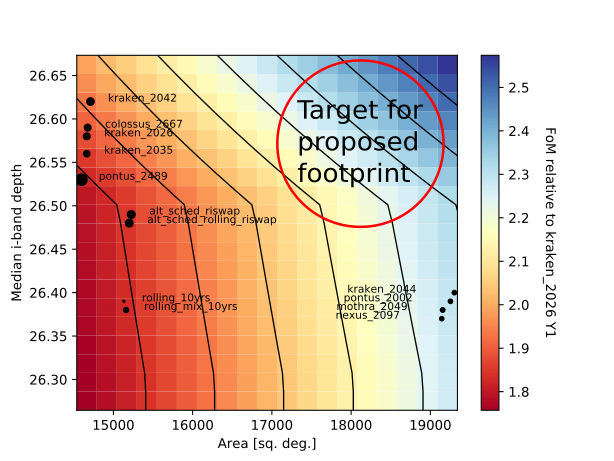
\includegraphics[width=0.7\columnwidth,  trim={0cm 0cm 0cm 0cm}, clip]{test_noprior_Y10_contour_text.png}
    \captionof{figure}{Emulated DETF FoM \emph{excluding systematics} \review{(as this is still a work in progress)} for the joint static science probes as a function of area and depth for Y10, relative to the FoM for \texttt{kraken\_2026} Y1. Points are scaled by a weak lensing systematic metric where larger circles are preferable. \review{Stage 3 priors are not included here.}
    }
    \label{fig:static_fom}
\end{minipage}

\begin{minipage}{0.99\columnwidth}
    \centering
    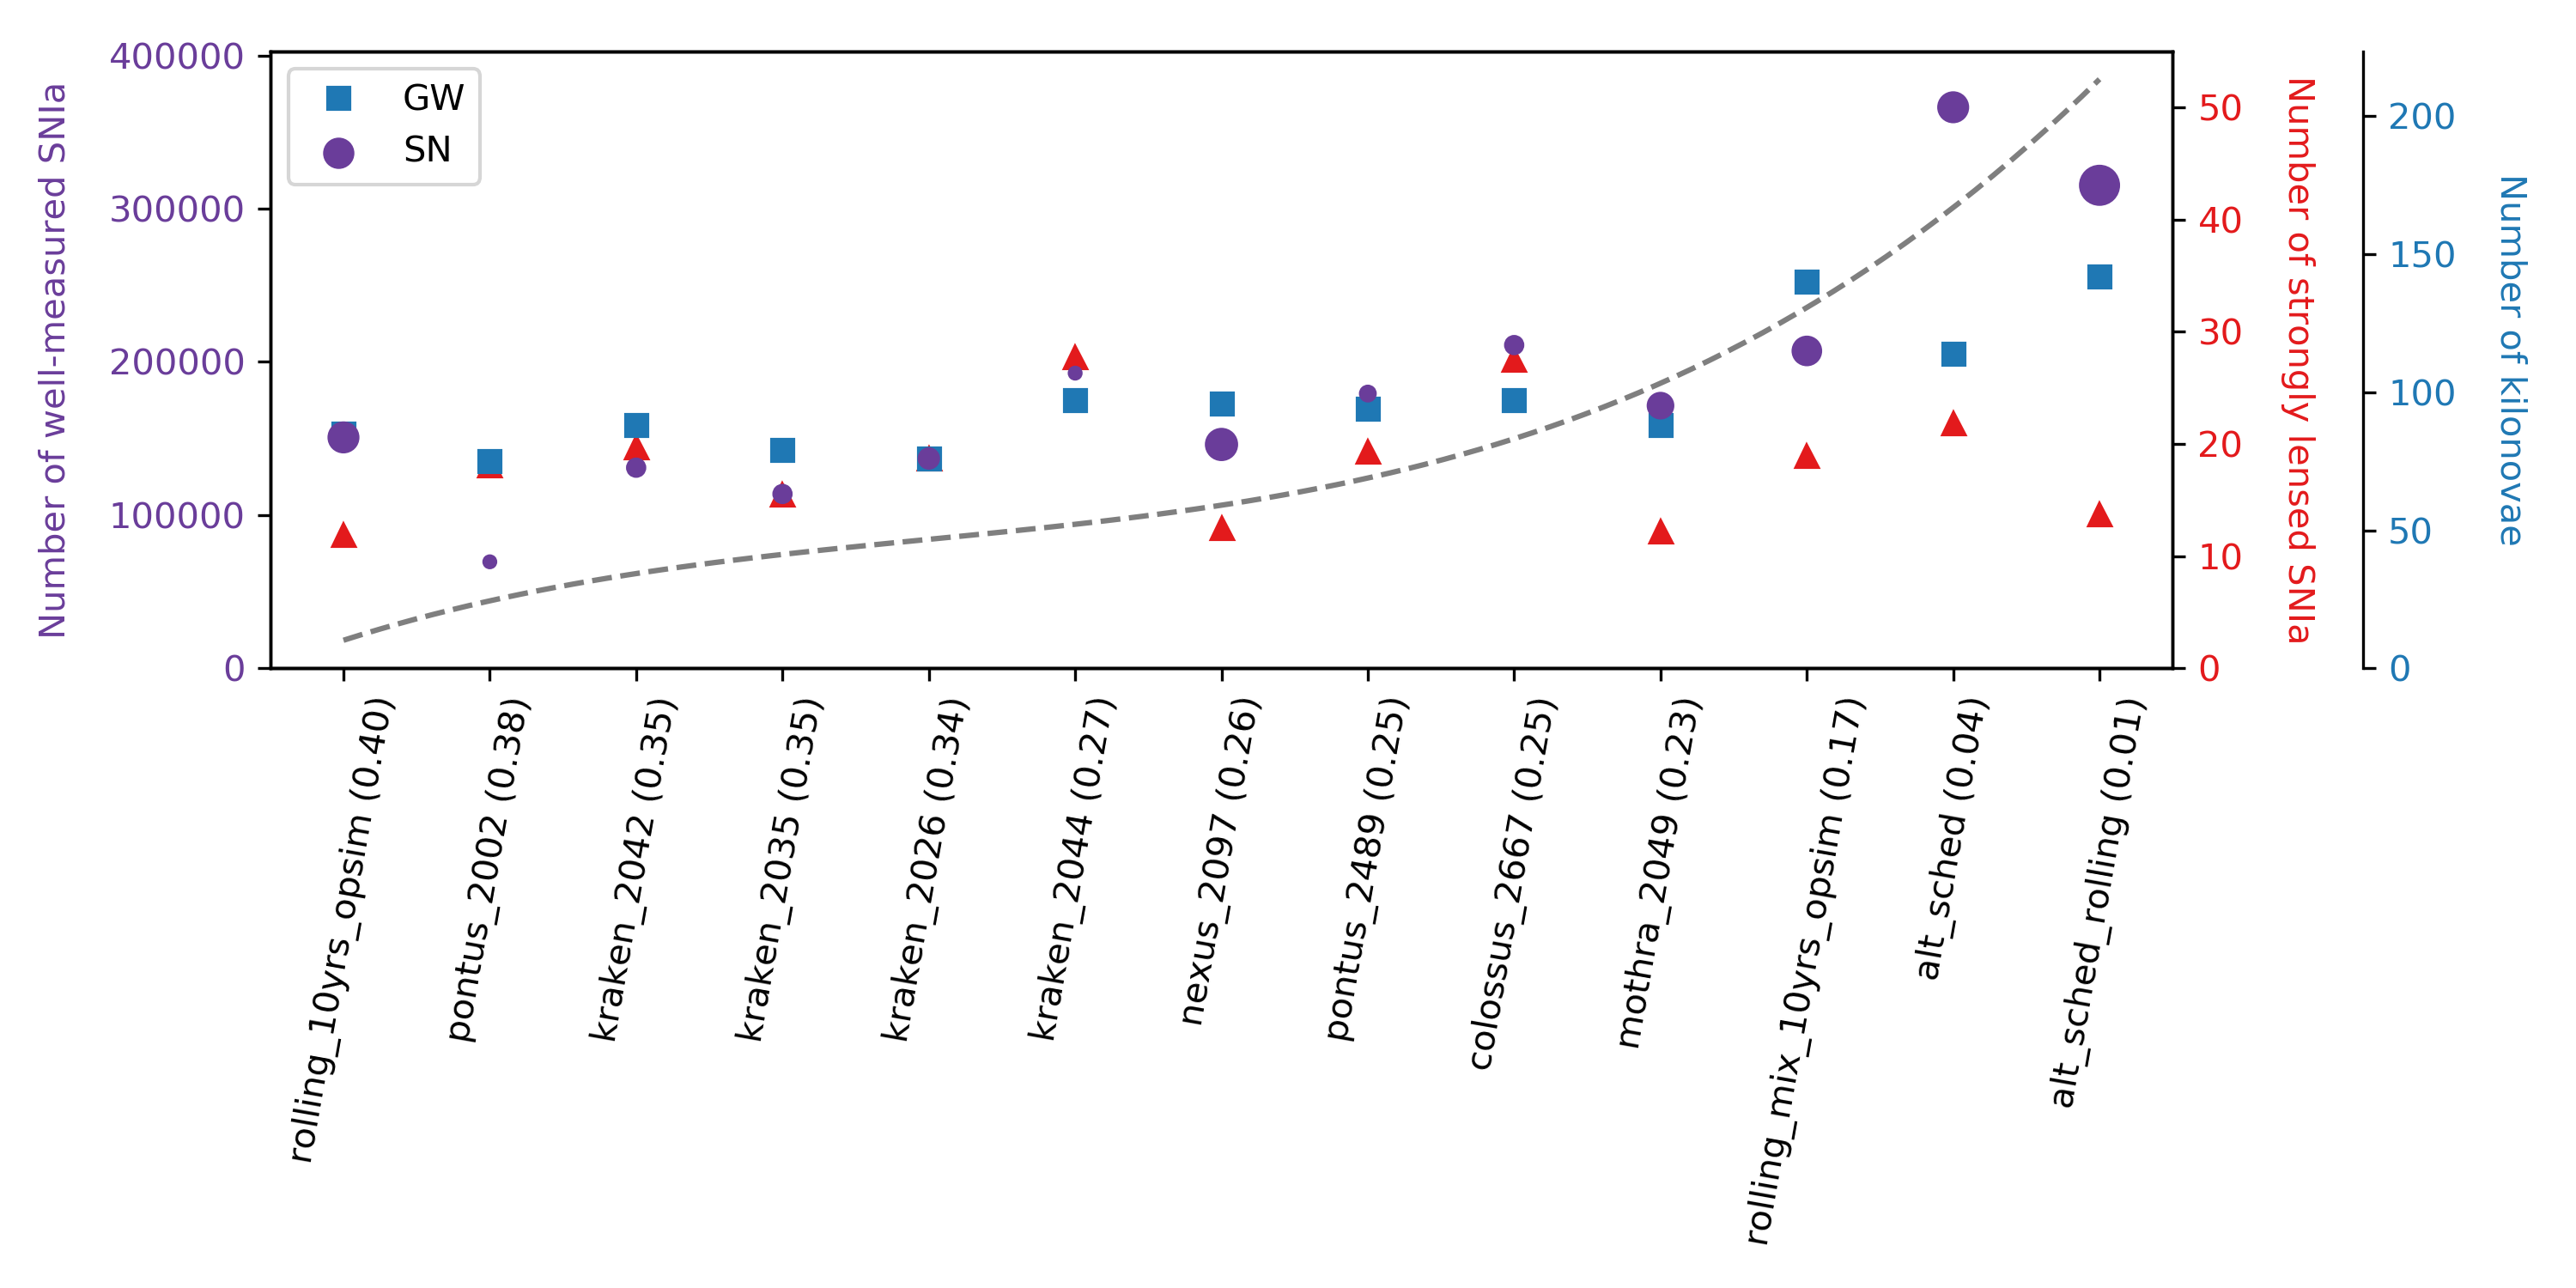
\includegraphics[width=0.99\columnwidth]{transients.png}
    \captionof{figure}{The number of kilonovae (GW), strongly lensed type Ia supernovae with well-measured time delays (SL) \reviewnew{(both assuming follow-up with other telescopes)} and well-measured type Ia supernovae (SN) as a function of observing strategy. The size of the points corresponding to number of well-measured supernovae are scaled by $z_{\rm{cut}}$. The strategies are ordered by the percentage of visits in $r$-band that are separated by more than 15 days
(number shown in brackets). The dashed line is a trend line (average in broad bins and splined) to guide the eye.  }
    \label{fig:transients}
\end{minipage}




% \subsection{Proxy Metrics}

% \subsubsection{Weak Lensing}
% {\bfseries Number of visits as a proxy for PSF estimation}\\
% One of the most important systematic effects in weak lensing is modeling of the point spread function. The detailed simulations and analysis of PSF modeling is outside the scope of this white paper, but it was found that the total number of visits is a good proxy for PSF estimation as more visits average down PSF error. It should be noted that this is only estimate of an important systematic, not a proxy for the performance of weak lensing as whole which is instead included in the DETF FoM described below.

% \subsubsection{Large Scale Structure}
% There are two important factors that affect large scale structure, weak lensing and clusters similarly: uniform area and depth. Described here are two metrics that work as proxies for the performance of all these probes.\\
% {\bfseries Total usable sky area}\\
% This is the sky area that achieves (after 10 years although interim years were also considered) a 5$\sigma$ depth of 26 in i-band, after applying an E(B-V)<0.2 cut and ensuring that there is coverage in all six filters (for photometric redshifts).\\
% {\bfseries Standard deviation of i-band 5$\sigma$ depth}\\
% This metric is a proxy for uniformity and is computed after the same cuts are applied that are used to compute the total usable area. A lower standard deviation implies better uniformity and thus less systematic effects.

% \subsubsection{Photometric Redshifts}
% {\bfseries Photo-z quality}\\
% We make use of the metric described in \cite{graham2017} to evaluate the impact of observing strategy on photometric redshifts. This is given by  $\Delta z_{(1+z)} = (z_{\rm{true}} − z_{\rm{phot}})/(1 + z_{\rm{phot}}))$.\\
% \ml{This isn't quite what was done, needs to be corrected!}



% \subsubsection{Supernovae}
% Cosmology with type Ia supernovae is heavily impacted by observing strategy. There are no simple metrics that can act as proxy since supernovae depend on a number of different survey strategy factors including depth, cadence, filter changes, filter distribution etc. We have developed a collection of metrics that consider many different aspects of supernova science. 
% {\bfseries Number of supernovae and median redshift}\\
% For this metric, a large sample of supernovae need to be simulated for a given strategy. These are then subject to several cuts: \\
% {\bfseries Peculiar velocities f$\sigma_8$}\\
% {\bfseries Photometric classification}\\
% {\bfseries Area overlap with 4MOST}\\

% \subsubsection{Strong Lensing}
% {\bfseries Number of LSNe Ia with LSST only}\\
% {\bfseries Number of LSNe Ia with LSST + follow up}\\

% \subsubsection{Gravitational Waves}
% {\bfseries Number of kilonovae with DES-GW model}\\
% {\bfseries Number of kilonovae with SAEE model}\\

% \subsection{DETF Figure of Merit}
% \subsubsection{Joint Static Science Analysis}
% \subsubsection{Supernovae}

\vspace{.6in}

\section{Special Data Processing}
% \begin{footnotesize}
% {\it Describe any data processing requirements beyond the standard LSST Data Management pipelines and how these will be achieved.}\\
% \end{footnotesize}

%EG added the following 
\review{We expect to reprocess $\sim$1\% of the data roughly 10 times, performed at NERSC and varying key DM Stack parameters.  This will allow analysis teams to estimate the impact of systematic uncertainties influenced by the reduction e.g., blending.  Hence our total reprocessing budget is roughly 10\% of each annual data release.}
  

\section{Requests for New OpSim Runs}
\label{sec:requests}
In the course of our study, we determined several factors that may impact cosmology but which require further investigation. Here we describe several new simulations we would like to request. We request that all DDFs and mini-surveys be simulated together to study the impact on WFD. 
\begin{itemize}
    \item {\bfseries Seeing prioritization:} Static science will benefit from reserving the best seeing conditions for $r$ and $i$ band, but this may negatively impact strong lensing that tends to observe bluer objects. We thus request one simulation with $r$,$i$ prioritized for best seeing and one with $g$,$r$, $i$ prioritized. 
    
    \item {\bfseries Variable exposure time:} We propose to allow exposure time to vary based on observing conditions (seeing, airmass, sky brightness \& transparency) to \review{improve single visit depth for transient detection and} achieve more uniform depth for galaxy detection/shape measurement. 
    %EG edited following sentences 
    We request that pairs of visits (which we argue should be in different filters) be kept to the same exposure time and that all visits be longer than 15s but less than 60s, even when atmospheric conditions are so good or poor to suggest otherwise. 
    
    \item {\bfseries Redistribution of filters:} We propose halving the number of visits in $y$-band and redistributing them. Figure 6 in \cite{graham2017} shows that while photometric redshifts are sensitive to changes in u-band depth, even halving the number of visits in $y$-band does not noticeably reduce photo-z quality. This may be one of the reasons why AltSched performs so well for supernovae. \review{However this effect must be further explored before we can understand the full impact on photometric redshifts.} Thus we would like to request simulations exploring the reduction of the number of visits in $y$-band by half and redistributing these to $gri$. The optimal filter distribution is unknown so multiple simulations would be appreciated.
    
    \item {\bfseries Clustered $u$ and  $y$  band visits:} Since $griz$ bands are \review{the most important} for our transient science cases, we request an observation which clusters (for example) all u-band and $y$-band visits in a month in a couple of nights (\review{i.e. making all $u$-band in a short sequence of dark nights and making $y$-band visits a few weeks later around bright time}), thus allowing $griz$ cadence to be improved in the intervening time. \review{The effectiveness of this approach will depend on how important the different filters are for early classification which is still under investigation.}
    
    \item{\bfseries Accurate seeing and weather:} In [Link to Eric Neilsen's paper], it was found that a more realistic seeing model has a large impact on LSST science, 
    and we recommend updating the seeing and weather models \review{(especially making some worst-case scenario weather simulations)} in the next round of simulations. \review{It would be interesting to consider strategies able to adapt in the event of poor weather.}
    
    \item{\bfseries Rolling cadence:} We would like to \review{work with the OpSim team to} continue investigating rolling cadence as a promising avenue to improve transient cosmology. In particular, we would be interested in a rolling cadence that achieves uniformity in years 1,3,6,10 and rolls in the intervening years, as well as rolling cadence options that maintain a low-level of uniform progression (e.g., 25\% of the baseline visits) in the deprioritized sky region.
    
    \item{\bfseries AltSched-like simulations:} The alternative scheduler to OpSim has shown impressive results for transient science due to its highly regular cadence in every filter (see \autoref{fig:transients}). We would thus request a simulation using OpSim, but with the same scheduling pattern as AltSched. This requires scanning the meridian, deviating only as necessary to increase season length. Observations should be taken in 45 minute blocks, incrementing the filter each revisit. The sky should be partitioned into two parts, observing each part on alternating nights. Ideally, the starting filter should be incremented by by 2 each night (e.g. from $u$ to $r$ or $g$ to $i$). 
    
    %EG's idea below, feel free to cut/modify if this is already handled elsewhere!  
    \item{\bfseries Dark-time mode:}  Instead of choosing which filters to image in based on dark vs. bright nights, we would like to simulate a strategy where the dark portions of otherwise bright nights are used for $g$ and $r$-band imaging of visit pairs.  This could help reduce the incidence of otherwise long gaps in the $g$-band coverage caused by lunar phase.  
    
\end{itemize}
\section{Acknowledgements}
 \begin{footnotesize}
This paper has undergone internal review in the LSST Dark Energy Science Collaboration. The authors are grateful to the internal reviewers who were Jonathan Blazek, Chihway Chang, Ariel Goobar, William Hartley Isobel Hook, Saurabh Jha, Nacho Sevilla Noarbe, Anže Slosar, Eli Rykoff and Peter Yoachim. 
 \end{footnotesize}
\section{References}
\bibliographystyle{hunsrt}
%Removes the extra section heading
\begingroup
\renewcommand{\section}[2]{}%
\bibliography{refs}
\endgroup


\end{document}
